Im ersten Schritt wird die Leerlaufspannung $U_\symup{0}$ einer Monozelle
gemessen. Hierfür werden die Anschlüsse des Voltmeters direkt mit den Anschlüssen
der Monozelle verbunden. Die angezeigt Spannung und der Innenwiderstand des
Voltmeters $R_\symup{i,V}$ werden notiert.
Nach dieser Messung werden ein Amperemeter und ein regelbarer Widerstand
$R_\symup{a}$ wie in \ref{fig:schlt1} mit der Monozelle in Reihe geschaltet.
\begin{figure}[H]
  \centering
  \begin{subfigure}{0.5\textwidth}
    \centering
    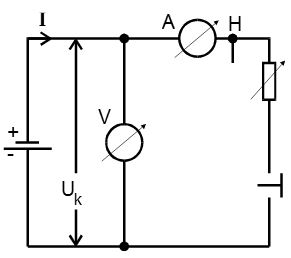
\includegraphics{bilder/sinrecht.jpg}
    \caption{Messreihe 1}
    \label{fig:schlt1}
  \end{subfigure}
  \begin{subfigure}{0.5\textwidth}
    \centering
    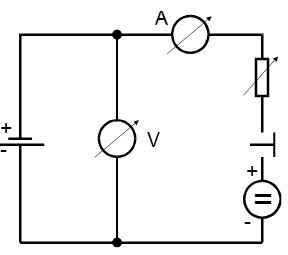
\includegraphics{bilder/gegenspannung.jpg}
    \caption{Messreihe 2}
    \label{fig:schlt2}
  \end{subfigure}
  \caption{Schaltbilder \cite{301}}
  \label{fig:schlt}
\end{figure}
Das Voltmeter bleibt parallel geschaltet um den Spannungsverlauf über der
Monozelle zu messen. Der Widerstand wird hierbei von $(0-50)\symup{\si{\ohm}}$
variiert.
